\section{Attention Variants}\label{sec:method:attention}

The encoder of \cref{sec:method:arch} uses standard self-attention, which treats a window as an unordered set of tokens and lets every pulse attend to every other pulse purely through learned query--key compatibility.
The only ordering or physical-relationship cue available to it is whatever the input features themselves carry, in particular the \gls{toa} entry of each \gls{pdw}.
A radar recording, however, has strong pairwise structure: two pulses that are close in time, share a carrier frequency, or have a similar pulse width are far more likely to originate from the same emitter or mode than an arbitrary pair.
This section describes two variants of the attention mechanism that make such structure explicit. Each is evaluated as a drop-in replacement for the \gls{mha} sub-layers of \cref{sec:method:arch}; their relative merit is reported in \cref{ch:experiments}.

Throughout, we write the attention logits of a single head over a window of $L$ pulses as
\begin{equation}\label{eq:method:attn_base}
  \mat{A} = \frac{\mat{Q}\mat{K}^{\top}}{\sqrt{d_k}},
  \qquad
  A_{ij} = \frac{\vect{q}_i^{\top}\vect{k}_j}{\sqrt{d_k}},
\end{equation}
where $\vect{q}_i$ and $\vect{k}_j$ are the query and key of pulses $i$ and $j$ and $d_k$ is the per-head dimension.
The attention weights are the row-wise softmax of $\mat{A}$, which then mixes the value vectors.

\subsection*{Physical attention bias}

The first variant adds a pairwise bias to the attention logits, computed from the physical parameters of each pulse pair.
The bias is built from the absolute pairwise differences of three coordinates: the \gls{toa} $t_n$ and the two horizontal incidence-direction components $u^{x}_n$ and $u^{y}_n$ of \cref{eq:method:aoa_cart}.
As in the rotary variant below, the vertical component $u^{z}_n$ is omitted because the latitude estimate is the one most corrupted by ground reflections and similar multipath effects.
For each coordinate $f$, the delta matrix $B^{(f)}_{ij} = |f_i - f_j|$ is superposed on the logits with a learnable scalar coefficient,
\begin{equation}\label{eq:method:attn_bias}
  A_{ij} = \frac{\vect{q}_i^{\top}\vect{k}_j}{\sqrt{d_k}} + \sum_{f} \lambda_f\, B^{(f)}_{ij},
  \qquad
  f \in \{t,\, u^{x},\, u^{y}\}.
\end{equation}
Each coefficient $\lambda_f$ is learned jointly with the rest of the network and belongs to a single head of a single attention sub-layer, so every head in every encoder block—throughout the shared trunk and both branches—carries its own set of three coefficients.
No kernel shape is imposed on the bias: a negative $\lambda_f$ pushes attention towards pulses that are close in that coordinate, a positive one towards distant pulses, and $\lambda_f = 0$ removes the cue entirely, so the model chooses the sign and strength of each cue during training instead of committing to a hand-tuned prior.
Using component-wise direction deltas rather than differences of raw angles also avoids the azimuth wrap-around problem noted in \cref{sec:method:data:norm}.
Because the coefficients are learned independently in each part of the network, the branches are free to allocate the cues differently; one may expect the deinterleaving branch to lean more heavily on the direction deltas—pulses from one emitter arrive from a nearly constant direction—while the shared trunk and the mode branch, whose target should be invariant to viewing geometry, suppress them.
Whether this allocation emerges is examined in \cref{ch:experiments}.
The construction mirrors the relative-position and content-independent biases used in language and graph transformers \parencite{shaw2018relative,ying2021graphormer}, specialised here to pulse parameters rather than token indices.

\subsection*{Rotary positional encoding}

The bias variant adjusts the logits after the query--key product is formed; the second variant instead builds positional information into the queries and keys themselves.
The query and key of pulse $i$ are obtained by linear projection of the hidden representation $\vect{h}_i$ that enters the attention sub-layer,
\begin{equation}\label{eq:method:qk_proj}
  \vect{q}_i = \mat{W}_q\vect{h}_i,
  \qquad
  \vect{k}_i = \mat{W}_k\vect{h}_i,
\end{equation}
with learnable matrices $\mat{W}_q, \mat{W}_k \in \R^{d_k \times d_{\mathrm{model}}}$ shared across positions in the head.
In the vanilla self-attention of \cref{eq:method:attn_base}, the attention logit is then simply their inner product
\begin{equation}\label{eq:method:attn_dot}
  \bigl\langle \vect{q}_i,\, \vect{k}_j \bigr\rangle
  = \vect{q}_i^{\top}\vect{k}_j
  = (\mat{W}_q\vect{h}_i)^{\top}(\mat{W}_k\vect{h}_j).
\end{equation}
\Gls{rope} leaves these projections unchanged and rotates the resulting vectors by a phase that depends on a scalar coordinate $p$ attached to each pulse.
Following \textcite{su2024roformer}, the query and key become functions $f_q(\vect{h}_i, p_i)$ and $f_k(\vect{h}_j, p_j)$ of both the hidden representation and that coordinate, and their inner product is required to depend on the coordinates only through their difference,
\begin{equation}\label{eq:method:rope_goal}
  \bigl\langle f_q(\vect{h}_i, p_i),\, f_k(\vect{h}_j, p_j) \bigr\rangle
  = g(\vect{h}_i, \vect{h}_j, p_j - p_i).
\end{equation}
In the original formulation the coordinate is the token index, $p_i = i$.
We instead attach raw pulse parameters, so that $p_j - p_i$ is a physical quantity---a time gap or a difference in a direction component---rather than an ordinal distance; this suits the irregularly sampled recordings of \cref{sec:method:data}, where consecutive indices may be microseconds or milliseconds apart.
The construction is introduced first for a single coordinate, then extended to several coordinates that share a head, and finally assigned to the trunk and branches of \cref{sec:method:arch}.

\subsubsection*{Single-coordinate rotation}

\Gls{rope} satisfies \cref{eq:method:rope_goal} by encoding one scalar coordinate as a phase applied to the whole head.
The $d_k$ dimensions of a head (assumed even) are grouped into $d_k/2$ two-dimensional planes, and the $m$-th plane is rotated by the angle $\gamma p\theta_m$, where $\theta_m$ is a per-plane angular frequency and $\gamma > 0$ a coordinate scale, both specified below.
Each plane uses the planar rotation matrix
\begin{equation}\label{eq:method:rope_2d}
  \mat{\Omega}(\phi) =
  \begin{bmatrix}
    \cos\phi & -\sin\phi \\
    \sin\phi & \phantom{-}\cos\phi
  \end{bmatrix}.
\end{equation}
Collecting the per-plane rotations into a single block-diagonal matrix of size $d_k \times d_k$ gives
\begin{equation}\label{eq:method:rope_block}
  \mat{R}(p)
  = \diag\!\bigl(
      \mat{\Omega}(\gamma p\theta_1),\,
      \mat{\Omega}(\gamma p\theta_2),\,
      \ldots,\,
      \mat{\Omega}(\gamma p\theta_{d_k/2})
    \bigr),
\end{equation}
or written out entry-wise,
\[
  \mat{R}(p) =
  {\scriptsize
  \begin{bmatrix}
    \cos\gamma p\theta_1 & -\sin\gamma p\theta_1 & 0 & 0 & \cdots & 0 & 0 \\
    \sin\gamma p\theta_1 & \phantom{-}\cos\gamma p\theta_1 & 0 & 0 & \cdots & 0 & 0 \\
    0 & 0 & \cos\gamma p\theta_2 & -\sin\gamma p\theta_2 & \cdots & 0 & 0 \\
    0 & 0 & \sin\gamma p\theta_2 & \phantom{-}\cos\gamma p\theta_2 & \cdots & 0 & 0 \\
    \vdots & \vdots & \vdots & \vdots & \ddots & \vdots & \vdots \\
    0 & 0 & 0 & 0 & \cdots & \cos\gamma p\theta_{d_k/2} & -\sin\gamma p\theta_{d_k/2} \\
    0 & 0 & 0 & 0 & \cdots & \sin\gamma p\theta_{d_k/2} & \phantom{-}\cos\gamma p\theta_{d_k/2}
  \end{bmatrix}.}
\]
The angular frequencies $\theta_m = b^{-2(m-1)/d_k}$, with a fixed base $b$ (we use $b = 10^4$, following \textcite{su2024roformer}), form a geometric progression that mirrors the wavelengths of the sinusoidal encoding of \textcite{vaswani2017attention}: fast-rotating planes resolve fine coordinate differences, slow-rotating planes capture coarse ones.
The scale $\gamma$ multiplies every frequency of the ladder uniformly and therefore sets how much relative phase one unit of coordinate difference produces.
In the original formulation no such factor is needed, because token indices advance in steps of exactly one; our coordinates are normalised physical quantities in $[0,1]$ whose typical differences depend on the quantity, so $\gamma$ is treated as a hyperparameter of the attached coordinate.
Its values are reported in \cref{ch:experiments}; the dependence of $\mat{R}$ on $\gamma$ is left implicit in the notation.
Applying $\mat{R}(p)$ after the projections of \cref{eq:method:qk_proj} yields
\begin{equation}\label{eq:method:rope_map}
  f_q(\vect{h}_i, p_i) = \mat{R}(p_i)\,\vect{q}_i = \mat{R}(p_i)\,\mat{W}_q\vect{h}_i,
  \qquad
  f_k(\vect{h}_j, p_j) = \mat{R}(p_j)\,\vect{k}_j = \mat{R}(p_j)\,\mat{W}_k\vect{h}_j,
\end{equation}
written $\tilde{\vect{q}}_i$ and $\tilde{\vect{k}}_j$ below; without the rotation, \cref{eq:method:rope_map} reduces to the vanilla case of \cref{eq:method:attn_dot}.

That this construction meets the design goal follows from one property of planar rotations: composing two of them subtracts their angles, $\mat{\Omega}(\phi)^{\top}\mat{\Omega}(\psi) = \mat{\Omega}(\psi - \phi)$, hence block-wise $\mat{R}(p_i)^{\top}\mat{R}(p_j) = \mat{R}(p_j - p_i)$ and
\begin{equation}\label{eq:method:rope}
  \bigl\langle \tilde{\vect{q}}_i,\, \tilde{\vect{k}}_j \bigr\rangle
    = \vect{q}_i^{\top}\,\mat{R}(p_j - p_i)\,\vect{k}_j
    = (\mat{W}_q\vect{h}_i)^{\top}\,\mat{R}(p_j - p_i)\,(\mat{W}_k\vect{h}_j),
\end{equation}
which is exactly the form required by \cref{eq:method:rope_goal}: each pulse is rotated by its absolute coordinate, yet the logit sees only the difference.
Setting $\mat{R}(p) = \mat{I}$ recovers the content-only inner product of \cref{eq:method:attn_dot}.
\Cref{fig:method:rope} illustrates this on a single plane: increasing the coordinate fans a vector around the circle at a fixed rate (left), while the phase enclosed between a rotated query and key---and hence their dot product---is set by the coordinate gap alone (right).

\subsubsection*{Multi-coordinate rotation}

A single head can also carry several coordinates at once by partitioning its $d_k/2$ planes into disjoint slices and rotating each slice by a different coordinate, following the multi-axis \gls{rope} used for vision transformers \parencite{heo2024ropevit}.
For two coordinates, the planes are split evenly into two slices of $d_k/4$ planes each, so the query (and likewise the key) decomposes into two half-head vectors
\begin{equation}\label{eq:method:rope_split}
  \vect{q}_i
  =
  \begin{bmatrix}
    \vect{q}_i^{(x)} \\
    \vect{q}_i^{(y)}
  \end{bmatrix},
  \qquad
  \vect{q}_i^{(x)},\, \vect{q}_i^{(y)} \in \R^{d_k/2}.
\end{equation}
Each half is rotated by its own single-coordinate matrix of the form \cref{eq:method:rope_block}, but built from only $d_k/4$ planes and its own scale:
\begin{equation}\label{eq:method:rope_sliced}
  \mat{R}^{\mathrm{em}}_n
  =
  \diag\!\bigl(
    \mat{R}^{(x)}(u^{x}_n),\;
    \mat{R}^{(y)}(u^{y}_n)
  \bigr),
\end{equation}
with $\mat{R}^{(x)}(u^{x}_n),\, \mat{R}^{(y)}(u^{y}_n) \in \R^{d_k/2 \times d_k/2}$ using scales $\gamma_{u^x}$ and $\gamma_{u^y}$ respectively.
The rotated query is therefore
\begin{equation}\label{eq:method:rope_sliced_q}
  \tilde{\vect{q}}_n
  =
  \mat{R}^{\mathrm{em}}_n\vect{q}_n
  =
  \begin{bmatrix}
    \mat{R}^{(x)}(u^{x}_n)\,\vect{q}_n^{(x)} \\
    \mat{R}^{(y)}(u^{y}_n)\,\vect{q}_n^{(y)}
  \end{bmatrix},
\end{equation}
and likewise for the key: each matrix acts only on its half of the head, never on the other coordinate's dimensions.
Applying the relative-phase identity of \cref{eq:method:rope} slice-wise then yields
\begin{equation}\label{eq:method:rope_sliced_logit}
  \bigl\langle \tilde{\vect{q}}_i,\, \tilde{\vect{k}}_j \bigr\rangle
    = \vect{q}_i^{(x)\top}\,\mat{R}^{(x)}\bigl(u^{x}_j - u^{x}_i\bigr)\,\vect{k}_j^{(x)}
    + \vect{q}_i^{(y)\top}\,\mat{R}^{(y)}\bigl(u^{y}_j - u^{y}_i\bigr)\,\vect{k}_j^{(y)}.
\end{equation}
The attention logit is the sum of two independent relative terms, one for each half of the head.
\Cref{fig:method:rope_slicing} contrasts this layout with the single-coordinate case.

\subsubsection*{Allocation across the encoder}

The coordinates considered are the \gls{toa} $t_n$ and the two horizontal direction components $u^{x}_n$ and $u^{y}_n$ of \cref{eq:method:aoa_cart}, normalised as in \cref{sec:method:data}.
The vertical component $u^{z}_n$ is not used as a rotation coordinate: it derives from the latitude angle, whose estimate is the one most corrupted by ground reflections and similar multipath effects, and omitting it leaves more planes for each retained coordinate under the multi-coordinate split.
It remains available to the model as a plain input feature (\cref{sec:method:data}).

The shared trunk and the mode branch use the single-coordinate form of \cref{eq:method:rope_block}: every plane of every head is rotated by the \gls{toa}, with scale $\gamma_t$.
Arrival direction is excluded there, because an operating mode is characterised by the intrinsic temporal pattern of the emission and must be recognised regardless of viewing geometry; rotating those layers by direction would inject nuisance variation into an embedding that should be geometry-invariant.

The deinterleaving branch instead uses the two-coordinate form of \cref{eq:method:rope_sliced}, rotating the two head halves by $u^{x}_n$ and $u^{y}_n$.
Direction is a strong cue for emitter identity---within a window, pulses from one emitter arrive from a nearly constant direction---while temporal structure is already present upstream, because every window passes through the \gls{toa}-rotated trunk before reaching the branch.
Repeating the \gls{toa} rotation in the branch would therefore spend half the head on a cue the representation already carries.
Cartesian direction components are used rather than a rescaled azimuth: because \gls{rope} turns coordinate differences into relative phases, rotating by azimuth would ignore the identification of $0$ with $2\pi$, so two pulses arriving from nearly the same direction could receive an almost maximal relative phase; differences of $u^{x}$ and $u^{y}$ vary continuously over the sphere.

This variant complements rather than replaces the bias term---the bias adds pairwise relationships to the logits, while \gls{rope} encodes coordinate differences in the geometry of the queries and keys---and it revisits the choice of \cref{sec:method:arch} to rely on \gls{toa} and arrival direction as plain input features, testing whether an explicit relative encoding adds information beyond their presence in the input.

\begin{figure}[tbp]
  \centering
  % =====================================================================
% Allocation of the d_k/2 rotation planes of one attention head to
% physical coordinates.  Top strip: in the shared trunk and the mode
% branch every plane is rotated by the TOA t_n
% (\cref{eq:method:rope_block}).  Bottom strip: in the deinterleaving
% branch the planes are split evenly into two slices of d_k/4 planes,
% rotated by the horizontal direction components u^x_n and u^y_n
% (\cref{eq:method:rope_sliced}).  Loaded from
% sections/04_method/04_attention_variants.tex via \input{...}.
% =====================================================================
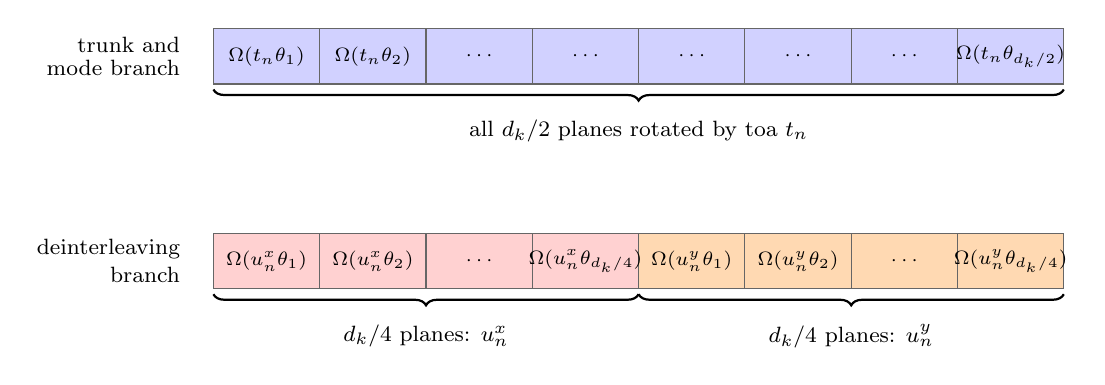
\begin{tikzpicture}[
    font=\small,
    plane/.style={draw=black!60, thin, minimum width=13.5mm, minimum height=7mm,
                  inner sep=0pt, outer sep=0pt},
    toaplane/.style={plane, fill=blue!18},
    uxplane/.style={plane, fill=red!18},
    uyplane/.style={plane, fill=orange!30},
    rowlabel/.style={font=\footnotesize, anchor=east},
    slicebrace/.style={decorate, decoration={brace, mirror, amplitude=4pt}, thick},
    bracelabel/.style={font=\footnotesize, anchor=north},
  ]

  \def\W{13.5mm}   % plane cell width
  \def\NP{8}    % number of plane cells drawn per strip

  % =================== TOP STRIP: trunk and mode branch =================
  \node[rowlabel] at (-3mm, 0) {\shortstack[r]{trunk and\\mode branch}};
  \foreach \m in {1,...,\NP} {
    \node[toaplane] (t\m) at ({(\m-0.5)*\W}, 0) {};
  }
  \node[font=\scriptsize] at (t1) {$\mat{\Omega}(t_n\theta_1)$};
  \node[font=\scriptsize] at (t2) {$\mat{\Omega}(t_n\theta_2)$};
  \node[font=\scriptsize] at (t3) {$\cdots$};
  \node[font=\scriptsize] at (t4) {$\cdots$};
  \node[font=\scriptsize] at (t5) {$\cdots$};
  \node[font=\scriptsize] at (t6) {$\cdots$};
  \node[font=\scriptsize] at (t7) {$\cdots$};
  \node[font=\scriptsize] at (t8) {$\mat{\Omega}(t_n\theta_{d_k/2})$};

  \draw[slicebrace] (0, -4.2mm) -- ({\NP*\W}, -4.2mm);
  \node[bracelabel] at ({\NP*\W/2}, -6.8mm)
    {all $d_k/2$ planes rotated by \gls{toa} $t_n$};

  % ============== BOTTOM STRIP: deinterleaving branch ====================
  \begin{scope}[yshift=-26mm]
    \node[rowlabel] at (-3mm, 0) {\shortstack[r]{deinterleaving\\branch}};
    \foreach \m in {1,...,4} {
      \node[uxplane] (b\m) at ({(\m-0.5)*\W}, 0) {};
    }
    \foreach \m in {5,...,8} {
      \node[uyplane] (b\m) at ({(\m-0.5)*\W}, 0) {};
    }
    \node[font=\scriptsize] at (b1) {$\mat{\Omega}(u^{x}_n\theta_1)$};
    \node[font=\scriptsize] at (b2) {$\mat{\Omega}(u^{x}_n\theta_2)$};
    \node[font=\scriptsize] at (b3) {$\cdots$};
    \node[font=\scriptsize] at (b4) {$\mat{\Omega}(u^{x}_n\theta_{d_k/4})$};
    \node[font=\scriptsize] at (b5) {$\mat{\Omega}(u^{y}_n\theta_1)$};
    \node[font=\scriptsize] at (b6) {$\mat{\Omega}(u^{y}_n\theta_2)$};
    \node[font=\scriptsize] at (b7) {$\cdots$};
    \node[font=\scriptsize] at (b8) {$\mat{\Omega}(u^{y}_n\theta_{d_k/4})$};

    \draw[slicebrace] (0, -4.2mm) -- ({4*\W}, -4.2mm);
    \node[bracelabel] at ({2*\W}, -6.8mm)
      {$d_k/4$ planes: $u^{x}_n$};

    \draw[slicebrace] ({4*\W}, -4.2mm) -- ({8*\W}, -4.2mm);
    \node[bracelabel] at ({6*\W}, -6.8mm)
      {$d_k/4$ planes: $u^{y}_n$};
  \end{scope}

\end{tikzpicture}

  \caption{Allocation of the $d_k/2$ rotation planes of one attention head. \emph{Top:} single-coordinate \gls{rope} in the shared trunk and mode branch---all planes rotated by the \gls{toa} $t_n$ with scale $\gamma_t$ (\cref{eq:method:rope_block}). \emph{Bottom:} multi-coordinate \gls{rope} in the deinterleaving branch---the planes are split into two slices of $d_k/4$ planes, rotated by $u^{x}_n$ and $u^{y}_n$ with scales $\gamma_{u^x}$ and $\gamma_{u^y}$ (\cref{eq:method:rope_sliced}); each matrix acts only on its half of the head (\cref{eq:method:rope_sliced_q,eq:method:rope_sliced_logit}). The \gls{toa} is not repeated in the branch because the trunk representations are already \gls{toa}-rotated. Ellipsis cells indicate intermediate planes of each frequency ladder.}
  \label{fig:method:rope_slicing}
\end{figure}

\begin{figure}[tbp]
  \centering
  % =====================================================================
% Geometry of RoPE on one 2D plane of an attention head.
% Left: projected query q is rotated by R(p) for two nearby physical
% coordinates (e.g. window-normalised TOA), with a modest phase
% gamma*p*theta_m (\cref{eq:method:rope_block}).
% Right: after both query and key are rotated, their enclosed angle
% (and hence the inner product) depends only on the coordinate
% difference (\cref{eq:method:rope}).
% Loaded from sections/04_method/04_attention_variants.tex via \input.
% =====================================================================
\begin{tikzpicture}[
    font=\small,
    >=Latex,
    axis/.style={->, gray!55, thin},
    guide/.style={gray!30, thin},
    qraw/.style={->, thick, densely dashed, color=black!50},
    qvec/.style={->, very thick, color=blue!70!black},
    kraw/.style={->, thick, densely dashed, color=red!45!black},
    kvec/.style={->, very thick, color=red!70!black},
    angarc/.style={->, thin, color=black!70},
    steparrow/.style={->, thick, color=black!55},
  ]

  % =================== LEFT PANEL: apply R(p) to the projected query ====
  \begin{scope}[xshift=0mm]
    \def\Rad{17mm}
    \node[font=\footnotesize\bfseries, anchor=south] at (0, 22mm)
      {Apply $\mat{R}(p)$ to the projected query};

    \draw[axis] (-20mm, 0) -- (21mm, 0);
    \draw[axis] (0, -7mm) -- (0, 20mm);
    \draw[guide] (0, 0) circle (\Rad);

    % modest angles: content at 20°, then +12° and +22° of phase
    \def\qbase{20}
    \def\aone{32}   % R(p_i) q : small absolute phase
    \def\atwo{42}   % R(p_j) q : slightly larger

    % unrotated projected query
    \draw[qraw] (0, 0) -- (\qbase:\Rad);
    \node[color=black!50, font=\scriptsize, anchor=north west]
      at (\qbase:\Rad) {$\vect{q}=\mat{W}_q\vect{h}$};

    % two gently rotated copies (nearby physical coordinates)
    \draw[qvec, color=blue!55!black] (0, 0) -- (\aone:\Rad);
    \draw[qvec] (0, 0) -- (\atwo:\Rad);

    \node[color=blue!55!black, font=\scriptsize, anchor=west]
      at (\aone:\Rad) {$\tilde{\vect{q}}(p_i)$};
    \node[color=blue!70!black, font=\scriptsize, anchor=south west]
      at (\atwo:\Rad) {$\tilde{\vect{q}}(p_j)$};

    % phase arc for the smaller rotation only
    \draw[angarc] (\qbase:8.5mm) arc (\qbase:\aone:8.5mm);
    \node[font=\scriptsize, anchor=west] at ({(\qbase+\aone)/2}:10mm)
      {$\gamma p_i\theta_m$};

    % annotation: what the diagram depicts
    \node[font=\scriptsize, anchor=north, align=center, text=black!65]
      at (0, -8mm)
      {$\tilde{\vect{q}}=\mat{R}(p)\,\vect{q}$\\[-1pt]
       nearby $p$ $\Rightarrow$ small relative phase};
  \end{scope}

  % =================== RIGHT PANEL: relative phase / inner product ======
  \begin{scope}[xshift=68mm]
    \def\Rad{17mm}
    \node[font=\footnotesize\bfseries, anchor=south] at (0, 22mm)
      {Inner product sees only $p_j-p_i$};

    \draw[axis] (-20mm, 0) -- (21mm, 0);
    \draw[axis] (0, -7mm) -- (0, 20mm);
    \draw[guide] (0, 0) circle (\Rad);

    % content angle between unrotated q and k (faint)
    \def\qrawang{18}
    \def\krawang{38}   % content angle φ = 20°
    % after relative rotation by gamma*(p_j-p_i)*theta_m ≈ 14°
    \def\qang{18}
    \def\kang{52}

    % faint unrotated pair (content-only geometry)
    \draw[qraw] (0, 0) -- (\qrawang:\Rad);
    \draw[kraw] (0, 0) -- (\krawang:\Rad);
    \node[color=black!45, font=\scriptsize, anchor=north west]
      at (\qrawang:0.92*\Rad) {$\vect{q}_i$};
    \node[color=red!40!black, font=\scriptsize, anchor=south east]
      at (\krawang:0.95*\Rad) {$\vect{k}_j$};

    % content-angle arc
    \draw[angarc, color=black!40] (\qrawang:6.5mm) arc (\qrawang:\krawang:6.5mm);
    \node[font=\scriptsize, color=black!50, anchor=west]
      at ({(\qrawang+\krawang)/2}:7.5mm) {$\varphi$};

    % bold rotated pair
    \draw[qvec] (0, 0) -- (\qang:\Rad);
    \draw[kvec] (0, 0) -- (\kang:\Rad);
    \node[color=blue!70!black, font=\scriptsize, anchor=west]
      at (\qang:\Rad) {$\tilde{\vect{q}}_i$};
    \node[color=red!70!black, font=\scriptsize, anchor=south west]
      at (\kang:\Rad) {$\tilde{\vect{k}}_j$};

    % relative-phase arc between rotated vectors
    \draw[angarc] (\qang:11mm) arc (\qang:\kang:11mm);
    \node[font=\scriptsize, anchor=south west]
      at ({(\qang+\kang)/2}:12.2mm)
      {$\varphi{+}\gamma(p_j{-}p_i)\theta_m$};

    \node[font=\scriptsize, anchor=north, align=center, text=black!65]
      at (0, -8mm)
      {$\langle\tilde{\vect{q}}_i,\tilde{\vect{k}}_j\rangle
        =\vect{q}_i^{\top}\mat{R}(p_j{-}p_i)\,\vect{k}_j$};
  \end{scope}

\end{tikzpicture}

  \caption{Geometry of single-coordinate \gls{rope} on one of the $d_k/2$ two-dimensional planes of a head. \emph{Left:} the projected query $\vect{q}=\mat{W}_q\vect{h}$ (dashed) is obtained exactly as in vanilla attention (\cref{eq:method:qk_proj}); \gls{rope} then applies the planar rotation $\mat{R}(p)$ of \cref{eq:method:rope_block}, adding a modest absolute phase $\gamma p\theta_m$. \emph{Right:} after both the query and the key are rotated, the enclosed angle equals the content angle $\varphi$ (dashed pair) plus the relative phase $\gamma(p_j-p_i)\theta_m$; the inner product therefore depends on the coordinate difference alone (\cref{eq:method:rope}).}
  \label{fig:method:rope}
\end{figure}
